
\documentclass[tikz]{standalone}

\usetikzlibrary{arrows.meta, fadings, graphs, shapes,
                decorations.markings, calc}

\tikzset{
  changeset/.style={
    draw=#1,
    thick,
    minimum width=3em,
    minimum height=2em
  },
  changeset/.default={black},
%
  obschangeset/.style={
    draw=#1,
    thick,
    dashed,
    minimum width=3em,
    minimum height=2em
  },
  obschangeset/.default={black},
%
  upperT/.style={
    fill=white,
    minimum width=0,
    minimum height=0,
  },
%
  tmpchangeset/.style={
    obschangeset,
    postaction={
      decorate,
      decoration={
        markings,
        mark=at position 0.5 with {\node[upperT] {\tiny{\textbf{T}}};},
      },
    },
  },
  tmpchangeset/.default={black},
%
  nodenote/.style={
    fill=red!20,
    line width=2mm
  },
%
  edge/.style={
    draw=#1,
    latex-,
    thick
  },
  edge/.default={black},
%
  obsedge/.style={
    draw=#1,
    latex-,
    thick
  },
  obsedge/.default={black},
%
  markeredge/.style={
    draw=#1,
    latex-,
    thick,
    dotted
  },
  markeredge/.default={black},
}

\begin{document}

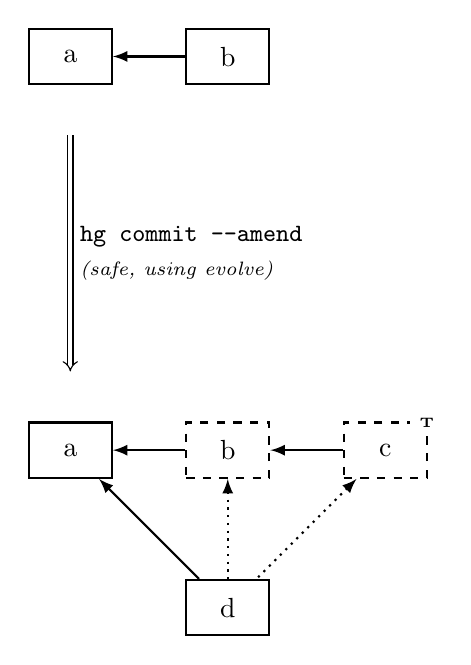
\begin{tikzpicture}

\node[changeset] at (4,-8) (d84) {d};
\node[obschangeset] at (4,-6) (b64) {b};
\node[tmpchangeset] at (6,-6) (c66) {c};
\node[changeset] at (2,-1) (a12) {a};
\node[changeset] at (2,-6) (a62) {a};
\node[changeset] at (4,-1) (b14) {b};
\draw[double, double equal sign distance, -Implies] (2,-2) -- node[anchor=west, align=left] (t33) {\small{\texttt{hg commit --amend}}\\\scriptsize\emph{(safe, using evolve)}} ++(0,-3);
\draw[edge] (a62) -- (d84);
\draw[markeredge] (b64) -- (d84);
\draw[markeredge] (c66) -- (d84);
\draw[edge] (a62) -- (b64);
\draw[edge] (b64) -- (c66);
\draw[edge] (a12) -- (b14);


\end{tikzpicture}
\end{document}

